% !TEX spellcheck = en_US



% ~~~~~~~~~~~~~~~~~~~~~~~~~~~~~~~~~~~~~~~ V
% (NC) 2026 Haluk Bingol
% github.com/halukbingol/LaTeX-Templates
%
% Licensees may copy, distribute, display, and perform the work and make derivative works 
% and remixes based on it only for non-commercial purposes. 
% ~~~~~~~~~~~~~~~~~~~~~~~~~~~~~~~~~~~~~~~ A




% =====================================================================
%  Unit Testing with JUnit -- Concepts
%  ---------------------------------------------------------------------
%  Built on hblib/Template/hblibTemplate.tex with the libraries in ../../hblib/.
%  Programs and their real outputs are in codeoutput/:
%     codeoutput/<Name>.java  a program (classes without main() are only compiled)
%     codeoutput/<Name>.sh    a terminal session, run in a copy of codeoutput/<Name>/
%     codeoutput/<Name>.txt   what it printed, made by:  bash run_examples.sh
% =====================================================================

\documentclass[aspectratio=169,10pt,compress]{beamer}

% ~~~~~~~~~~~~~~~~~~~~~~~~~~~~~~~~~~~~~~~~~~~~~~~~~~~~~~~~~~~~~~~~~ V hblib
	\usepackage{../../hblib/hblibPresentation} % lib presentation: theme, i/N, \hSection, algorithm2e, ...
	\usepackage{../../hblib/hblibCodeoutput} % lib code + output: \lstcode, \lstterminal, ...
	\usepackage{../../hblib/hblibDatastructures} % lib data structures: \hString, \hStack, \hQueue
% ~~~~~~~~~~~~~~~~~~~~~~~~~~~~~~~~~~~~~~~~~~~~~~~~~~~~~~~~~~~~~~~~~ A hblib


% theme, i/N, fonts (T1, lmodern), booktabs, xcolor, array (L{width} columns), listings, tikz,
% algorithm2e (\small captions, \Fn) and the color gitred come from the hblib libraries




% +++++++++++++++++++++++++++++++++++++++ V specific
\DontPrintSemicolon % in algorithms
\newcommand{\win}{\textbf{Windows}}
\newcommand{\mac}{\textbf{macOS}}
% +++++++++++++++++++++++++++++++++++++++ A specific

% ---------------------------------------------------------------------
\title{Unit Testing with JUnit}
\subtitle{Concepts}
\author[Bingol]{Haluk O. Bingol}

\institute[FCIS]{
    Faculty of Computer and Information Sciences\\
    Yeditepe University
}
\date{
	{\tiny \hbTimeStamp}
}

\begin{document}




% ~~~~~~~~~~~~~~~~~~~~~~~~~~~~~~~~~~~~~~ V frm
\begin{frame}[t,fragile]
  \titlepage
\end{frame}
% ~~~~~~~~~~~~~~~~~~~~~~~~~~~~~~~~~~~~~~ A frm




% ~~~~~~~~~~~~~~~~~~~~~~~~~~~~~~~~~~~~~~ V frm
\begin{frame}[t,fragile] \frametitle{Outline}
  \begin{columns}[T]
    \begin{column}{0.48\textwidth}
      \tableofcontents[sections={1-4}, hideallsubsections]
    \end{column}
    \begin{column}{0.48\textwidth}
      \tableofcontents[sections={5-8}, hideallsubsections]
    \end{column}
  \end{columns}
\end{frame}
% ~~~~~~~~~~~~~~~~~~~~~~~~~~~~~~~~~~~~~~ A frm

% ~~~~~~~~~~~~~~~~~~~~~~~~~~~~~~~~~~~~~~ V
\hSection[Why]{Why Automated Tests?}
% ~~~~~~~~~~~~~~~~~~~~~~~~~~~~~~~~~~~~~~ A




% ~~~~~~~~~~~~~~~~~~~~~~~~~~~~~~~~~~~~~~ V frm
\begin{frame}[t,fragile] \frametitle{A bug costs more the later it is found}
  \begin{columns}[T]
    \begin{column}{0.5\textwidth}
      \begin{center}
      \begin{tikzpicture}[x=1.1cm, y=0.5cm]
        \draw[-latex] (0,0) -- (5.4,0) node[right, font=\scriptsize] {time};
        \draw[-latex] (0,0) -- (0,5.5) node[above, font=\scriptsize] {cost of a fix};
        \foreach \x/\h/\l in {0.6/0.4/typing, 1.6/0.9/test, 2.6/1.8/review, 3.6/3.2/release, 4.6/5/user}
          {\fill[colorHEmph] (\x-0.3,0) rectangle (\x+0.3,\h);
           \node[font=\scriptsize, below] at (\x,0) {\l};}
      \end{tikzpicture}
      \end{center}
    \end{column}
    \begin{column}{0.46\textwidth}
      \begin{itemize}\small
        \item A bug found by a test minutes after typing costs minutes; found by a user, it costs days and trust.
        \item \textbf{Regression}: a change breaks something that used to work. Only re-running all tests catches it.
        \item Tests are also \textbf{documentation}: they show how the code is meant to be used.
        \item They make \textbf{change} safe: refactor without fear.
      \end{itemize}
    \end{column}
  \end{columns}
\end{frame}
% ~~~~~~~~~~~~~~~~~~~~~~~~~~~~~~~~~~~~~~ A frm

% ~~~~~~~~~~~~~~~~~~~~~~~~~~~~~~~~~~~~~~ V
\hSection[Levels]{Kinds of Tests}
% ~~~~~~~~~~~~~~~~~~~~~~~~~~~~~~~~~~~~~~ A




% ~~~~~~~~~~~~~~~~~~~~~~~~~~~~~~~~~~~~~~ V frm
\begin{frame}[t,fragile] \frametitle{From a method to the whole system}
  \begin{columns}[T]
    \begin{column}{0.46\textwidth}
      \begin{center}
      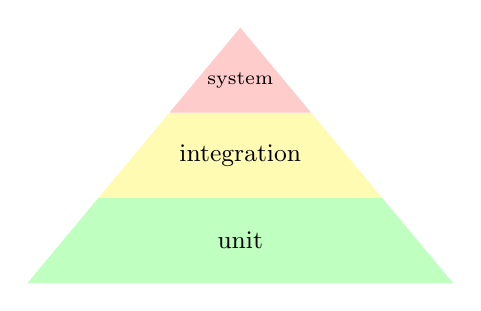
\begin{tikzpicture}[scale=0.9]
        \fill[green!25] (-3,0) -- (3,0) -- (2,1.2) -- (-2,1.2) -- cycle;
        \fill[yellow!30] (-2,1.2) -- (2,1.2) -- (1,2.4) -- (-1,2.4) -- cycle;
        \fill[red!20] (-1,2.4) -- (1,2.4) -- (0,3.6) -- cycle;
        \node[font=\small] at (0,0.6) {unit};
        \node[font=\small] at (0,1.8) {integration};
        \node[font=\scriptsize] at (0,2.85) {system};
      \end{tikzpicture}
      \end{center}
    \end{column}
    \begin{column}{0.5\textwidth}
      \begin{center}\small
      \begin{tabular}{lll}
        \toprule
        \textbf{level} & \textbf{tests}               & \textbf{speed} \\
        \midrule
        unit           & one class or method          & ms \\
        integration    & classes + database, files    & seconds \\
        system         & the whole program            & minutes \\
        acceptance     & what the customer asked for  & minutes \\
        \bottomrule
      \end{tabular}
      \end{center}
      \small The \textbf{pyramid}: many fast unit tests at the bottom, few slow system tests at the top.
      JUnit is mostly used for unit and integration tests.
    \end{column}
  \end{columns}
\end{frame}
% ~~~~~~~~~~~~~~~~~~~~~~~~~~~~~~~~~~~~~~ A frm

% ~~~~~~~~~~~~~~~~~~~~~~~~~~~~~~~~~~~~~~ V
\hSection[Anatomy]{Anatomy of a Unit Test}
% ~~~~~~~~~~~~~~~~~~~~~~~~~~~~~~~~~~~~~~ A




% ~~~~~~~~~~~~~~~~~~~~~~~~~~~~~~~~~~~~~~ V frm
\begin{frame}[t,fragile] \frametitle{Arrange, act, assert}
  \begin{columns}[T]
    \begin{column}{0.5\textwidth}
      \lstcode[basicstyle=\ttfamily\scriptsize]{codeoutput/Taste/PriceTest.java}{Java}
    \end{column}
    \begin{column}{0.46\textwidth}
      \begin{itemize}\small
        \item \textbf{Test method}: \texttt{@Test}, no parameters, no return value.
        \item \textbf{Arrange}: prepare the input (here: 100).
        \item \textbf{Act}: call the code under test (\texttt{withVat}).
        \item \textbf{Assert}: compare with the \textbf{expected} value (120); stop with a message if different.
      \end{itemize}
      \uncover<2->{\lstterminal[basicstyle=\ttfamily\tiny]{codeoutput/Taste.txt}}
    \end{column}
  \end{columns}
\end{frame}
% ~~~~~~~~~~~~~~~~~~~~~~~~~~~~~~~~~~~~~~ A frm




% ~~~~~~~~~~~~~~~~~~~~~~~~~~~~~~~~~~~~~~ V frm
\begin{frame}[t,fragile] \frametitle{Words of the trade}
  \begin{center}\small
  \begin{tabular}{lL{0.66\textwidth}}
    \toprule
    \textbf{term}       & \textbf{meaning} \\
    \midrule
    code under test     & the class or method being checked \\
    test case           & one scenario: input, action, expected result \\
    assertion           & a check: \emph{expected} versus \emph{actual} \\
    fixture             & the objects and data a test starts from \\
    test suite          & a set of tests run together \\
    test runner         & the program that finds, runs and reports tests \\
    test double         & a stand-in for a collaborator: stub, fake, mock, spy \\
    \bottomrule
  \end{tabular}
  \end{center}
\end{frame}
% ~~~~~~~~~~~~~~~~~~~~~~~~~~~~~~~~~~~~~~ A frm

% ~~~~~~~~~~~~~~~~~~~~~~~~~~~~~~~~~~~~~~ V
\hSection[JUnit]{JUnit}
% ~~~~~~~~~~~~~~~~~~~~~~~~~~~~~~~~~~~~~~ A




% ~~~~~~~~~~~~~~~~~~~~~~~~~~~~~~~~~~~~~~ V frm
\begin{frame}[t,fragile] \frametitle{JUnit: history and parts}
  \begin{columns}[T]
    \begin{column}{0.5\textwidth}
    	JUnit Home: junit.org~\cite{homeJunit}
      \begin{center}\small
      \begin{tabular}{lll}
        \toprule
        \textbf{year} & \textbf{version} & \textbf{new} \\
        \midrule
        1997          & JUnit 1--3       & Kent Beck and Erich Gamma \\
        2006          & JUnit 4          & annotations: \texttt{@Test} \\
        2017          & JUnit 5          & Platform + Jupiter, lambdas \\
        2025          & JUnit 6          & Java 17, one version number \\
        \bottomrule
      \end{tabular}
      \end{center}
      \vspace{0.3em}
      \begin{itemize}\small
        \item Free, open source; the standard for Java. Current: \textbf{6.1.3}.
        \item The idea spread to every language: pytest, NUnit, Jest, \dots{} (``xUnit'').
      \end{itemize}
    \end{column}
    \begin{column}{0.46\textwidth}
      \begin{center}
      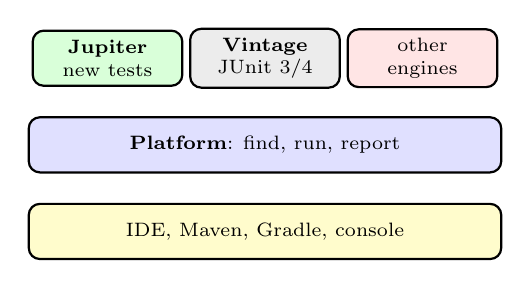
\begin{tikzpicture}[b/.style={draw, thick, rounded corners, minimum width=1.9cm, minimum height=0.7cm, font=\scriptsize, align=center}]
        \node[b, fill=blue!12, minimum width=6cm] (p) at (0,0) {\textbf{Platform}: find, run, report};
        \node[b, fill=green!15] at (-2,1.1) {\textbf{Jupiter}\\ new tests};
        \node[b, fill=gray!15]  at (0,1.1)  {\textbf{Vintage}\\ JUnit 3/4};
        \node[b, fill=red!10]   at (2,1.1)  {other\\ engines};
        \node[b, fill=yellow!20, minimum width=6cm] at (0,-1.1) {IDE, Maven, Gradle, console};
      \end{tikzpicture}
      \end{center}
      \small Tools speak to the Platform; \textbf{engines} run a kind of test. Our tests are \textbf{Jupiter} tests.
    \end{column}
  \end{columns}
\end{frame}
% ~~~~~~~~~~~~~~~~~~~~~~~~~~~~~~~~~~~~~~ A frm




% ~~~~~~~~~~~~~~~~~~~~~~~~~~~~~~~~~~~~~~ V frm
\begin{frame}[t,fragile] \frametitle{How a test class is run}
  \begin{columns}[T]
    \begin{column}{0.54\textwidth}
      \SetAlFnt{\small}


% +++++++++++++++++++++++++++++++++++++++ V alg
%: -Alg. 
\begin{algorithm}[H]
  \caption{Running one test class (Jupiter)}
  \KwIn{a class $C$ with test methods $t_{1}, \dots, t_{n}$}
  run the \texttt{@BeforeAll} methods\;
  \ForEach{test method $t_{i}$}{
    create a \textbf{new} object of $C$\;
    run the \texttt{@BeforeEach} methods\;
    run $t_{i}$; record passed / failed / aborted\;
    run the \texttt{@AfterEach} methods\;
  }
  run the \texttt{@AfterAll} methods\;
\end{algorithm}
% +++++++++++++++++++++++++++++++++++++++ A alg

    \end{column}
    \begin{column}{0.42\textwidth}
      \begin{itemize}\small
        \item A new object per test: tests cannot leak state through fields.
        \item \texttt{@BeforeAll}: expensive setup once (e.g.\ start a server).
        \item The order of $t_{1}, \dots, t_{n}$ is fixed but deliberately not obvious: tests must not depend on it.
      \end{itemize}
    \end{column}
  \end{columns}
\end{frame}
% ~~~~~~~~~~~~~~~~~~~~~~~~~~~~~~~~~~~~~~ A frm

% ~~~~~~~~~~~~~~~~~~~~~~~~~~~~~~~~~~~~~~ V
\hSection[Outcomes]{Outcomes and Assertions}
% ~~~~~~~~~~~~~~~~~~~~~~~~~~~~~~~~~~~~~~ A




% ~~~~~~~~~~~~~~~~~~~~~~~~~~~~~~~~~~~~~~ V frm
\begin{frame}[t,fragile] \frametitle{Four outcomes}
  \begin{center}\small
  \begin{tabular}{llL{0.5\textwidth}}
    \toprule
    \textbf{outcome} & \textbf{IDE}          & \textbf{cause} \\
    \midrule
    passed           & green                 & the method ended normally \\
    failed           & red                   & an assertion failed, or any other exception was thrown \\
    aborted          & yellow / gray         & an \textbf{assumption} did not hold (e.g.\ ``only on \win'') \\
    skipped          & gray                  & \texttt{@Disabled} or a condition, with a reason \\
    \bottomrule
  \end{tabular}
  \end{center}
  \begin{itemize}\small
    \item An \textbf{assertion} checks the result: \texttt{assertEquals}, \texttt{assertTrue}, \texttt{assertThrows}, \dots
    \item An \textbf{assumption} checks the environment: if it does not hold, the test is not meaningful here.
    \item ``0 tests found'' is not success: something is wrong with the setup.
  \end{itemize}
\end{frame}
% ~~~~~~~~~~~~~~~~~~~~~~~~~~~~~~~~~~~~~~ A frm

% ~~~~~~~~~~~~~~~~~~~~~~~~~~~~~~~~~~~~~~ V
\hSection[Good tests]{Good Tests}
% ~~~~~~~~~~~~~~~~~~~~~~~~~~~~~~~~~~~~~~ A




% ~~~~~~~~~~~~~~~~~~~~~~~~~~~~~~~~~~~~~~ V frm
\begin{frame}[t,fragile] \frametitle{FIRST and test doubles}
  \begin{columns}[T]
    \begin{column}{0.48\textwidth}
      \begin{center}\small
      \begin{tabular}{lL{0.6\linewidth}}
        \toprule
        \textbf{F}ast            & run them all the time \\
        \textbf{I}ndependent     & any order, any subset \\
        \textbf{R}epeatable      & same result anywhere \\
        \textbf{S}elf-validating & pass or fail by itself \\
        \textbf{T}imely          & written with the code \\
        \bottomrule
      \end{tabular}
      \end{center}
    \end{column}
    \begin{column}{0.48\textwidth}
      \begin{center}
      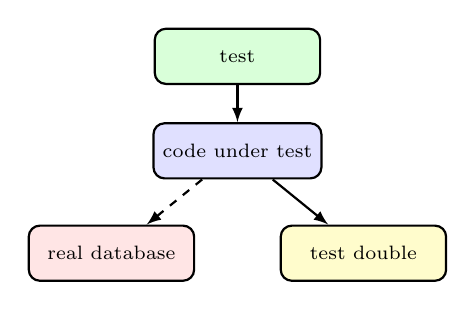
\begin{tikzpicture}[b/.style={draw, thick, rounded corners, minimum width=2.1cm, minimum height=0.7cm, font=\scriptsize, align=center}]
        \node[b, fill=green!15] (t) at (0,1.6) {test};
        \node[b, fill=blue!12] (c) at (0,0.4) {code under test};
        \node[b, fill=red!10] (db) at (-1.6,-0.9) {real database};
        \node[b, fill=yellow!20] (f) at (1.6,-0.9) {test double};
        \draw[-latex, thick] (t) -- (c);
        \draw[-latex, thick, dashed] (c) -- (db);
        \draw[-latex, thick] (c) -- (f);
      \end{tikzpicture}
      \end{center}
      \small Slow or unpredictable collaborators (database, network, clock, e-mail) are replaced by \textbf{test doubles}.
    \end{column}
  \end{columns}
\end{frame}
% ~~~~~~~~~~~~~~~~~~~~~~~~~~~~~~~~~~~~~~ A frm

% ~~~~~~~~~~~~~~~~~~~~~~~~~~~~~~~~~~~~~~ V
\hSection[TDD]{Test-Driven Development and Coverage}
% ~~~~~~~~~~~~~~~~~~~~~~~~~~~~~~~~~~~~~~ A




% ~~~~~~~~~~~~~~~~~~~~~~~~~~~~~~~~~~~~~~ V frm
\begin{frame}[t,fragile] \frametitle{Red, green, refactor}
  \begin{columns}[T]
    \begin{column}{0.46\textwidth}
      \begin{center}
      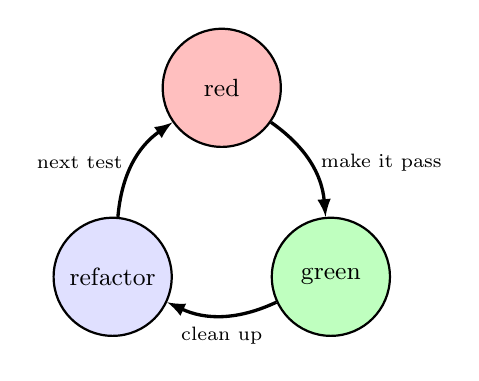
\begin{tikzpicture}[s/.style={circle, draw, thick, minimum size=1.5cm, font=\small, align=center}]
        \node[s, fill=red!25]   (r) at (90:1.6)  {red};
        \node[s, fill=green!25] (g) at (-30:1.6) {green};
        \node[s, fill=blue!12]  (f) at (210:1.6) {refactor};
        \draw[-latex, very thick] (r) to[bend left=25] node[right, font=\scriptsize] {make it pass} (g);
        \draw[-latex, very thick] (g) to[bend left=25] node[below, font=\scriptsize] {clean up} (f);
        \draw[-latex, very thick] (f) to[bend left=25] node[left, font=\scriptsize] {next test} (r);
      \end{tikzpicture}
      \end{center}
    \end{column}
    \begin{column}{0.5\textwidth}
      \begin{enumerate}\small
        \item \textbf{Red}: write a test for the next small behavior; see it fail.
        \item \textbf{Green}: write the simplest code that passes.
        \item \textbf{Refactor}: improve the code; the tests stay green.
      \end{enumerate}
      \small Tests written first are written from the \emph{requirement}, not from the code.
    \end{column}
  \end{columns}
\end{frame}
% ~~~~~~~~~~~~~~~~~~~~~~~~~~~~~~~~~~~~~~ A frm




% ~~~~~~~~~~~~~~~~~~~~~~~~~~~~~~~~~~~~~~ V frm
\begin{frame}[t,fragile] \frametitle{How good are the tests?}
  \begin{columns}[T]
    \begin{column}{0.48\textwidth}
      \begin{block}{Coverage}
        \small Which lines and branches ran during the tests (tool: JaCoCo).
        Low coverage shows untested code. High coverage does \textbf{not} show good tests: a test without
        assertions covers code too.
      \end{block}
    \end{column}
    \begin{column}{0.48\textwidth}
      \begin{block}{Mutation testing}
        \small A tool makes small bugs on purpose (\texttt{>=} becomes \texttt{>}) and runs the tests.
        A good test suite \emph{kills} each mutant by failing (tool: PIT).
      \end{block}
    \end{column}
  \end{columns}
\end{frame}
% ~~~~~~~~~~~~~~~~~~~~~~~~~~~~~~~~~~~~~~ A frm

% ~~~~~~~~~~~~~~~~~~~~~~~~~~~~~~~~~~~~~~ V
\hSection[Summary]{Summary}
% ~~~~~~~~~~~~~~~~~~~~~~~~~~~~~~~~~~~~~~ A




% ~~~~~~~~~~~~~~~~~~~~~~~~~~~~~~~~~~~~~~ V frm
\begin{frame}[t,fragile] \frametitle{Big ideas}
  \begin{itemize}
    \item Automated tests find bugs early, catch regressions, document behavior and make change safe.
    \item A unit test: arrange, act, assert; one behavior; fast and independent.
    \item JUnit: the Platform runs engines; Jupiter is the engine for JUnit 5 and 6 tests.
    \item A new object per test; \texttt{@BeforeEach} prepares the fixture.
    \item Outcomes: passed, failed, aborted, skipped.
    \item TDD: red, green, refactor. Coverage finds gaps; mutation testing measures strength.
  \end{itemize}
\end{frame}
% ~~~~~~~~~~~~~~~~~~~~~~~~~~~~~~~~~~~~~~ A frm




% ~~~~~~~~~~~~~~~~~~~~~~~~~~~~~~~~~~~~~~ V frm
\begin{frame}[t,fragile] \frametitle{Questions to think about}
  \begin{enumerate}\small
    \item Why is ``0 tests found, 0 failed'' not a good result?
    \item Why does JUnit create a new test object for every test method?
    \item Give an example of a test that is not \emph{repeatable}. How would you fix it?
    \item A method has 100\% coverage but a bug. How is that possible?
    \item Which is easier to test: a method that prints its result or one that returns it? Why?
  \end{enumerate}
\end{frame}
% ~~~~~~~~~~~~~~~~~~~~~~~~~~~~~~~~~~~~~~ A frm



% ~~~~~~~~~~~~~~~~~~~~~~~~~~~~~~~~~~~~~~ V References bib
\begin{frame}[t,allowframebreaks]\frametitle{References}
	\setbeamertemplate{bibliography item}[text] % sets numbers in references
%	\bibliographystyle{abbrv}
%	\bibliographystyle{apalike}
%	\bibliographystyle{ieeetr}
	\bibliographystyle{IEEEtran}
	%
	\tiny\bibliography{../../hblib/hblibDataStructures} % bib file	
\end{frame}
% ~~~~~~~~~~~~~~~~~~~~~~~~~~~~~~~~~~~~~~ A References bib




% ~~~~~~~~~~~~~~~~~~~~~~~~~~~~~~~~~~~~~~ V frm
\begin{frame}[t,fragile]
	\begin{center}
		\vspace{4cm}
		\hRemark{\Huge Questions?}
	\end{center}
\end{frame}
% ~~~~~~~~~~~~~~~~~~~~~~~~~~~~~~~~~~~~~~ A frm



\end{document}
